%%%%%%%%%%%%%%%%%%%%%%%%%%%%%%%%%%%%%%%%%
% Lachaise Assignment
% LaTeX Template
% Version 1.0 (26/6/2018)
%
% This template originates from:
% http://www.LaTeXTemplates.com
%
% Authors:
% Marion Lachaise & François Févotte
% Vel (vel@LaTeXTemplates.com)
%
% License:
% CC BY-NC-SA 3.0 (http://creativecommons.org/licenses/by-nc-sa/3.0/)
% 
%%%%%%%%%%%%%%%%%%%%%%%%%%%%%%%%%%%%%%%%%

%----------------------------------------------------------------------------------------
%	PACKAGES AND OTHER DOCUMENT CONFIGURATIONS
%----------------------------------------------------------------------------------------

\documentclass{article}

%%%%%%%%%%%%%%%%%%%%%%%%%%%%%%%%%%%%%%%%%
% Lachaise Assignment
% Structure Specification File
% Version 1.0 (26/6/2018)
%
% This template originates from:
% http://www.LaTeXTemplates.com
%
% Authors:
% Marion Lachaise & François Févotte
% Vel (vel@LaTeXTemplates.com)
%
% License:
% CC BY-NC-SA 3.0 (http://creativecommons.org/licenses/by-nc-sa/3.0/)
% 
%%%%%%%%%%%%%%%%%%%%%%%%%%%%%%%%%%%%%%%%%

%------------------------------------------%
% 		PARTE NOSSA 
%------------------------------------------%

\usepackage[portuguese]{babel}	

%----------------------------------------------------------------------------------------
%	PACKAGES AND OTHER DOCUMENT CONFIGURATIONS
%----------------------------------------------------------------------------------------


\usepackage{amsmath,amsfonts,stmaryrd,amssymb} % Math packages

\usepackage{enumerate} % Custom item numbers for enumerations

\usepackage[ruled]{algorithm2e} % Algorithms

\usepackage[framemethod=tikz]{mdframed} % Allows defining custom boxed/framed environments

\usepackage{listings} % File listings, with syntax highlighting
\lstset{
	basicstyle=\ttfamily, % Typeset listings in monospace font
}

%----------------------------------------------------------------------------------------
%	DOCUMENT MARGINS
%----------------------------------------------------------------------------------------

\usepackage{geometry} % Required for adjusting page dimensions and margins

\geometry{
	paper=a4paper, % Paper size, change to letterpaper for US letter size
	top=2.5cm, % Top margin
	bottom=3cm, % Bottom margin
	left=2.5cm, % Left margin
	right=2.5cm, % Right margin
	headheight=14pt, % Header height
	footskip=1.5cm, % Space from the bottom margin to the baseline of the footer
	headsep=1.2cm, % Space from the top margin to the baseline of the header
	%showframe, % Uncomment to show how the type block is set on the page
}

%----------------------------------------------------------------------------------------
%	FONTS
%----------------------------------------------------------------------------------------

\usepackage[utf8]{inputenc} % Required for inputting international characters
\usepackage[T1]{fontenc} % Output font encoding for international characters

\usepackage{XCharter} % Use the XCharter fonts

%----------------------------------------------------------------------------------------
%	COMMAND LINE ENVIRONMENT
%----------------------------------------------------------------------------------------

% Usage:
% \begin{commandline}
%	\begin{verbatim}
%		$ ls
%		
%		Applications	Desktop	...
%	\end{verbatim}
% \end{commandline}

\mdfdefinestyle{commandline}{
	leftmargin=10pt,
	rightmargin=10pt,
	innerleftmargin=15pt,
	middlelinecolor=black!50!white,
	middlelinewidth=2pt,
	frametitlerule=false,
	backgroundcolor=black!5!white,
	frametitle={Command Line},
	frametitlefont={\normalfont\sffamily\color{white}\hspace{-1em}},
	frametitlebackgroundcolor=black!50!white,
	nobreak,
}

% Define a custom environment for command-line snapshots
\newenvironment{commandline}{
	\medskip
	\begin{mdframed}[style=commandline]
}{
	\end{mdframed}
	\medskip
}

%----------------------------------------------------------------------------------------
%	FILE CONTENTS ENVIRONMENT
%----------------------------------------------------------------------------------------

% Usage:
% \begin{file}[optional filename, defaults to "File"]
%	File contents, for example, with a listings environment
% \end{file}

\mdfdefinestyle{file}{
	innertopmargin=1.6\baselineskip,
	innerbottommargin=0.8\baselineskip,
	topline=false, bottomline=false,
	leftline=false, rightline=false,
	leftmargin=2cm,
	rightmargin=2cm,
	singleextra={%
		\draw[fill=black!10!white](P)++(0,-1.2em)rectangle(P-|O);
		\node[anchor=north west]
		at(P-|O){\ttfamily\mdfilename};
		%
		\def\l{3em}
		\draw(O-|P)++(-\l,0)--++(\l,\l)--(P)--(P-|O)--(O)--cycle;
		\draw(O-|P)++(-\l,0)--++(0,\l)--++(\l,0);
	},
	nobreak,
}

% Define a custom environment for file contents
\newenvironment{file}[1][File]{ % Set the default filename to "File"
	\medskip
	\newcommand{\mdfilename}{#1}
	\begin{mdframed}[style=file]
}{
	\end{mdframed}
	\medskip
}

%----------------------------------------------------------------------------------------
%	NUMBERED QUESTIONS ENVIRONMENT
%----------------------------------------------------------------------------------------

% Usage:
% \begin{question}[optional title]
%	Question contents
% \end{question}

\mdfdefinestyle{question}{
	innertopmargin=1.2\baselineskip,
	innerbottommargin=0.8\baselineskip,
	roundcorner=5pt,
	nobreak,
	singleextra={%
		\draw(P-|O)node[xshift=1em,anchor=west,fill=white,draw,rounded corners=5pt]{%
		Question \theQuestion\questionTitle};
	},
}

\newcounter{Question} % Stores the current question number that gets iterated with each new question

% Define a custom environment for numbered questions
\newenvironment{question}[1][\unskip]{
	\bigskip
	\stepcounter{Question}
	\newcommand{\questionTitle}{~#1}
	\begin{mdframed}[style=question]
}{
	\end{mdframed}
	\medskip
}

%----------------------------------------------------------------------------------------
%	WARNING TEXT ENVIRONMENT
%----------------------------------------------------------------------------------------

% Usage:
% \begin{warn}[optional title, defaults to "Warning:"]
%	Contents
% \end{warn}

\mdfdefinestyle{warning}{
	topline=false, bottomline=false,
	leftline=false, rightline=false,
	nobreak,
	singleextra={%
		\draw(P-|O)++(-0.5em,0)node(tmp1){};
		\draw(P-|O)++(0.5em,0)node(tmp2){};
		\fill[black,rotate around={45:(P-|O)}](tmp1)rectangle(tmp2);
		\node at(P-|O){\color{white}\scriptsize\bf !};
		\draw[very thick](P-|O)++(0,-1em)--(O);%--(O-|P);
	}
}

% Define a custom environment for warning text
\newenvironment{warn}[1][Warning:]{ % Set the default warning to "Warning:"
	\medskip
	\begin{mdframed}[style=warning]
		\noindent{\textbf{#1}}
}{
	\end{mdframed}
}

%----------------------------------------------------------------------------------------
%	INFORMATION ENVIRONMENT
%----------------------------------------------------------------------------------------

% Usage:
% \begin{info}[optional title, defaults to "Info:"]
% 	contents
% 	\end{info}

\mdfdefinestyle{info}{%
	topline=false, bottomline=false,
	leftline=false, rightline=false,
	nobreak,
	singleextra={%
		\fill[black](P-|O)circle[radius=0.4em];
		\node at(P-|O){\color{white}\scriptsize\bf i};
		\draw[very thick](P-|O)++(0,-0.8em)--(O);%--(O-|P);
	}
}

% Define a custom environment for information
\newenvironment{info}[1][Info:]{ % Set the default title to "Info:"
	\medskip
	\begin{mdframed}[style=info]
		\noindent{\textbf{#1}}
}{
	\end{mdframed}
}
 % Include the file specifying the document structure and custom commands

%----------------------------------------------------------------------------------------
%	ASSIGNMENT INFORMATION
%----------------------------------------------------------------------------------------

\title{Computação Gráfica: Etapa\#1} % Title of the assignment

\author{Bernardo Rodrigues\\ \texttt{a79008@alunos.uminho.pt}\\ \and César Silva\\ \texttt{a77518@alunos.uminho.pt}\\ \and Pedro Faria\\ \texttt{a82725@alunos.uminho.pt} \and Rui Silva\\ \texttt{a77219@alunos.uminho.pt}\\} % Author name and email address

\date{Universidade do Minho --- \today} % University, school and/or department name(s) and a date

%----------------------------------------------------------------------------------------

\begin{document}

\maketitle 
\begin{figure}[H]
	\centering
	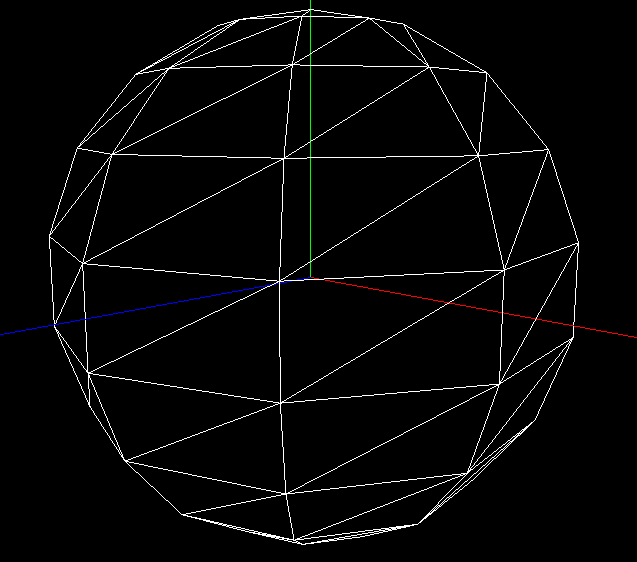
\includegraphics[width=6cm,height=6cm]{esfera}
\end{figure}
\newpage

\begin{abstract}
A \textbf{Computação Gráfica}, uma das muitas áreas da informática, que assume um papel fulcral em interações homem-máquina e na visualização de dados. o seu espectro de aplicações varia desde geração de imagens até a simulação do mundo real. \par
	O presente relatório refere-se às diferentes fases de entrega da componente prática da Unidade Curricular de \textbf{Computação Gráfica} enquadrada no curso de \textit{Ciências da Computação} da \textit{Universidade do Minho}. 
\end{abstract}
\newpage

%-------------------------------------------------
% 		METER A QUOTE AQUI
%-------------------------------------------------

\tableofcontents{}
\newpage

%-------------------------------------------------
%		Introducao
%-------------------------------------------------


\subsection{Estrutura do Relatório}
O presente documento divide-se em duas partes principais. A primeira onde expomos brevemente os conteúdos do trabalho, explicamos funcionalidades, fazemos considerações importantes e demonstração de resultados.
No fim, em anexo dispomos  todo o código interveniente dos diferentes módulos do projeto. 
\newpage

\section{Introdução}
Na primeira fase, foram desenvolvidas duas aplicações. Um \textbf{Gerador} de modelos, que aceite argumentos a partir do terminal, com a função de gerar os pontos de uma primitiva gráfica desejada pelo utilizador, imprimindo estes para um ficheiro. E a última, um \textbf{Motor} que interpreta os pontos gerados anteriormente de acordo com um ficheiro de configuração dado. 
Com base nos tópicos enunciados e ferramentas exploradas nas aulas implementamos o \textbf{Gerador} e o \textbf{Motor} na linguagem \textbf{C++}. Em particular esta última faz uso de biblioteca \textbf{TinyXML2} para que a leitura dos documentos que lhe são dados com input seja feita de forma simples e consistente. E por fim,  utilizamos a API fornecida pelo \textbf{OpenGl} para dar vida aos nossos modelos.\\
Na segunda, adicionamos features ao parser de ficheiros de configuração de \textbf{scenes}, nomeadamente, o reconhecimento de \textbf{scenes} dispostas hierarquicamente usando transformações geométricas (translações, rotações e de escala).
\newpage

\section{Fase 1}

\subsection{Gerador}
O nosso \textbf{Gerador} é um pequeno programa em \textbf{C++}, cuja implementação é disponibilizada em anexo, que depois de compilado, o correspondente executável escreve para um ficheiro (um por linha) os vértices da primitiva gráfica desejada  como iremos ilustrar nas seguintes secções.


\subsection{Caixa}
Para geração desta primitiva o utilizador deverá invocar a aplicação a com o nome do executável seguido dos comprimentos dos lados de um paraleloipipedo no eixos com X’s, Y’s e Z’s respetivamente e por fim o nome do ficheiro destino. A sintaxe é demonstrada no exemplo abaixo:

\begin{commandline}
    \begin{verbatim}
        $ g++ -o gerador gen.cpp
        $ ./gerador caixa 3 4 5 osmeusvertices
        $ ls
        $ gen.cpp            gerador            osmeusvertices.txt
    \end{verbatim}
\end{commandline}

\begin{figure}[H]
	\centering
	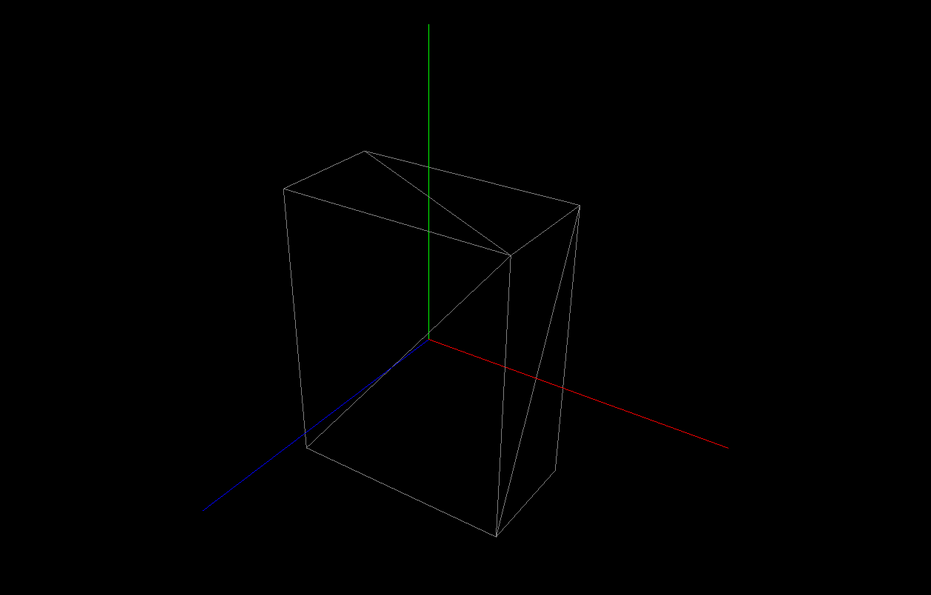
\includegraphics[width=4cm,height=4cm]{caixa}
	\caption{Caixa}
\end{figure}

\begin{warn}[Notice:]
Todas as faces são desenhadas com dois triângulos apontados para o exterior pela norma da mão direita mencionada nas aulas. Um zoom excessivo, ou a escolha de dimensões superiores à distância da câmara à origem(onde este é centrado)  pode levar ao aparente desaparecimento do modelo.
\end{warn}

\subsection{Cone}
O \textbf{Cone} recebe como argumentos o raio da base, a sua altura, o número de slices e stacks. \\
A construção deste começa por fixar um uma \textit{slice} calculando os vértices da base correspondente, de seguida todas as \textit{stacks} relativas, sendo o última stack - a do bico - um caso especial. \\
O algoritmo usa noções como semelhança de triângulos para cálculo dos sucessivos raios das circuferências formadas pelas \textit{stacks}.\\

\begin{info}
	Apresentamos o significado das variáveis usadas no programa que gera os pontos do \textbf{Cone}: 
	\begin{itemize}
		\item[] \textit{stkd} - diferença entre stacks consecutivas
		\item[] \textit{slcd} - diferença entre slices consecutivas
		\item[] \textit{raiod} - diferença entre o raio de duas stacks consecutivas
		\item[] \textit{stk} - stack atual 
		\item[] \textit{slc} - slice atual
		\item[] \textit{nslc} - próxima slice
		\item[] \textit{nstk} - próxima stack
		\item[] \textit{nr} - próximo raio
		\item[] \textit{r} - raio atual
	\end{itemize}
\end{info}

\begin{figure}[H]
	\centering
	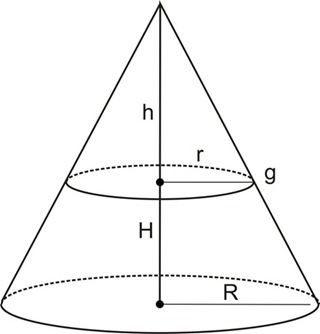
\includegraphics[width=4cm,height=4cm]{conesemelhante}
	\caption{Semelhança de triângulos num cone}
\end{figure}

Apresentamos algumas imagens que ilustram a criação do cone. \\

\begin{figure}[H]
	\centering
	\subfloat[2 stacks]{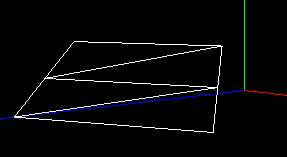
\includegraphics[width=3cm,height=3cm]{2stk}}
	\hspace{2cm}
	\subfloat[4 stacks]{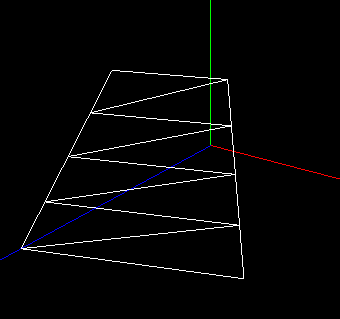
\includegraphics[width=3cm,height=3cm]{4stk}}
	\caption{Progessão das stacks do cone}
\end{figure}

\begin{figure}[H]
	\centering
	\subfloat[1 slice]{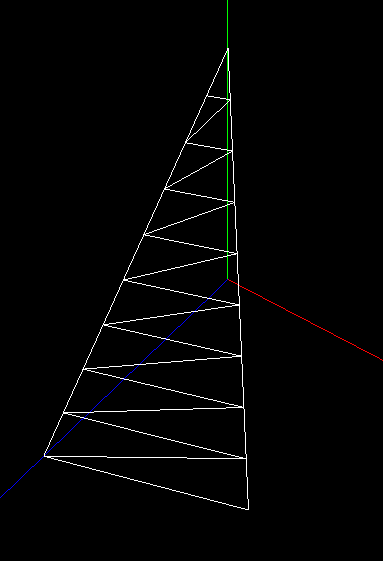
\includegraphics[width=3cm,height=3cm]{1slc}}
	\hspace{2cm}
	\subfloat[2 slices]{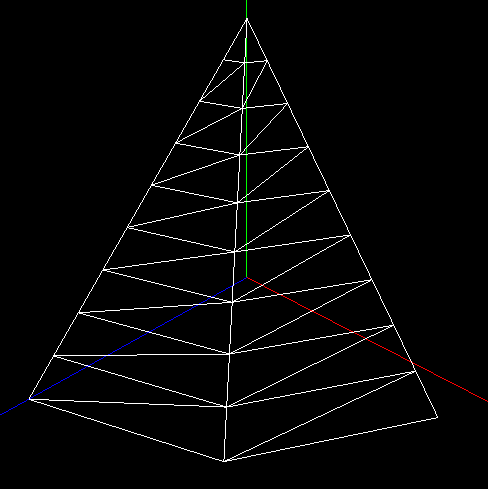
\includegraphics[width=3cm,height=3cm]{2slc}}
	\caption{Progessão das slices do cone}
\end{figure}

Finalmente obtemos:

\begin{figure}[H]
	\centering
	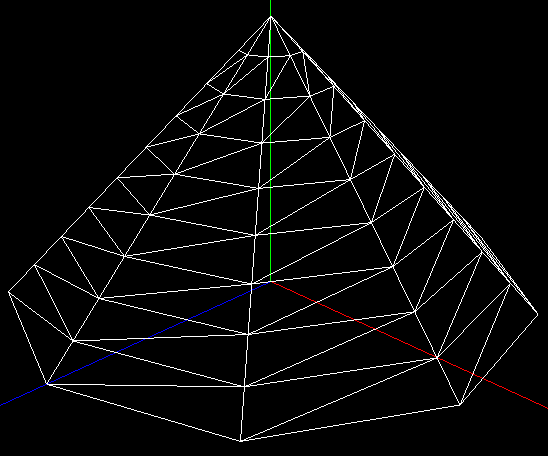
\includegraphics[width=4cm,height=4cm]{cone}
	\caption{Cone}
\end{figure}

\subsection{Esfera}
A \textbf{Esfera} recebe como argumentos o seu raio, o número de slices e stacks.
A sua construção usa coordenadas esféricas usando o raio dado como argumentos e manipulando 2 ângulos \textit{Alfa} e \textit{Beta}. \textit{Alfa} é dado por: \\
\[ alfa = \frac{2\times \Pi}{slices} \]
Este nos programas é usado juntamente com o raio para calcular os pontos de \textit{slices} consecutivas. De seguida \textit{beta} é dado por:\\
\[ beta = \frac{\Pi \div 2}{stacks}\] \\
Este desenpenha uma função igual ao anterior considerando \textit{stacks}.\\


\begin{figure}[H]
	\centering
	\subfloat[4 stacks]{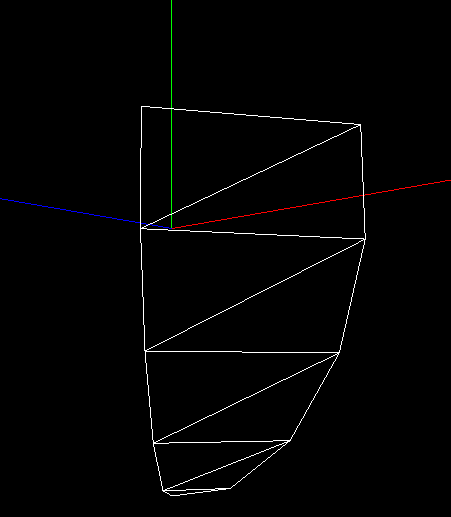
\includegraphics[width=3cm,height=3cm]{4estk}}
	\hspace{2cm}
	\subfloat[8 stacks]{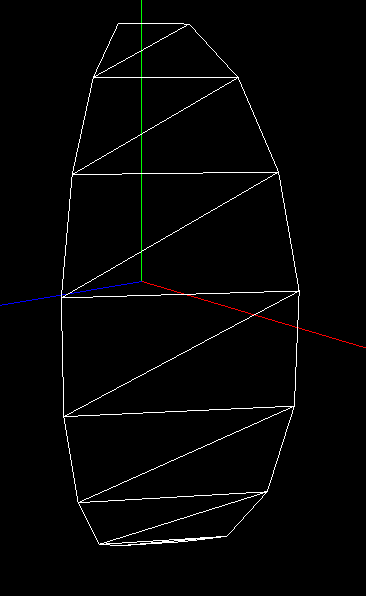
\includegraphics[width=3cm,height=3cm]{8estk}}
	\caption{Progessão das stacks da esfera}
\end{figure}

\begin{figure}[H]
	\centering
	\subfloat[1 slice]{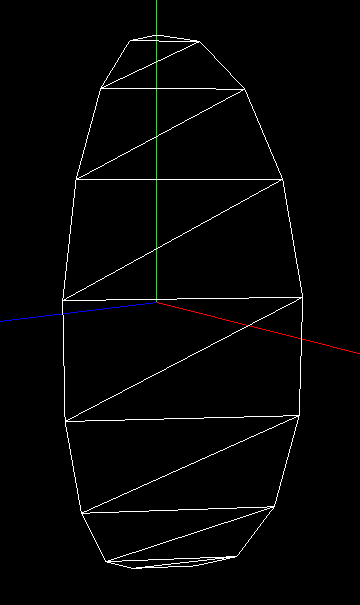
\includegraphics[width=3cm,height=3cm]{1eslc}}
	\hspace{2cm}
	\subfloat[2 slices]{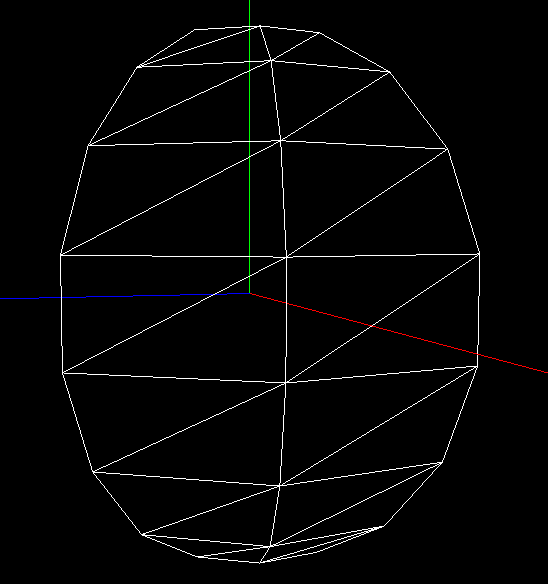
\includegraphics[width=3cm,height=3cm]{2eslc}}
	\caption{Progessão das slices da esfera}
\end{figure}

\begin{figure}[H]
	\centering
	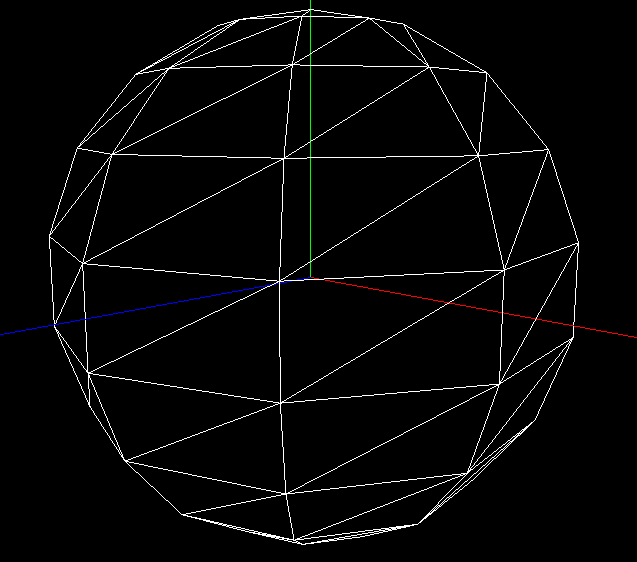
\includegraphics[width=4cm,height=4cm]{esfera}
	\caption{Esfera}
\end{figure}

\subsection{Plano}
O requisito estabelecido no guião do trabalho veio em muito simplificar a representação do plano XZ ao ponto de para a sua computação seja apenas necessário um único argumento que representa o tamanho da porção visível desejada.  

\begin{commandline}
    \begin{verbatim}
        $ g++ -o gerador gen.cpp
        $ ./gerador plano 5 pontos
        $ ls
        $ gen.cpp            gerador            pontos.txt
    \end{verbatim}
\end{commandline}

\begin{figure}[H]
	\centering
	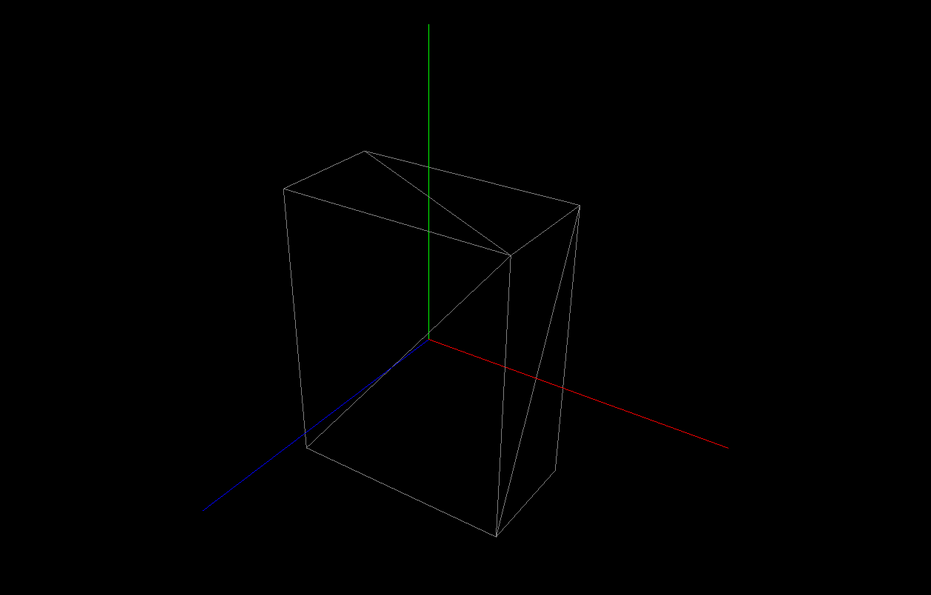
\includegraphics[width=4cm,height=4cm]{caixa}
	\caption{Caixa}
\end{figure}

\begin{warn}[Notice:]
Os planos são infinitos a referência ao tamanho é feita apenas para facilitar a observação do mesmo.
São desenhados 4 triângulos, em vez de dois, para que esta primitiva seja visível de todas as perspectivas.
\end{warn}

\newpage
\section{Motor}
O motor é a parte do nosso trabalho que faz o linking de todas as outras partes que foram realizadas. O motor, lê um ficheiro xml (conf.xml). Este ficheiro contém uma estrutura bastante simples, dividida em scenes.

% Contents do ficheiro conf.xml
\begin{file}[conf.xml]
	\begin{lstlisting}[language=XML]
	<scene>
		<model file="esfera.txt" />
		<model file="cone.txt" />
		<model file="caixa.txt" />
	</scene>
	\end{lstlisting}
	\end{file}

Cada ficheiro que está referenciado nas tags \textbf{<model>} é um ficheiro de texto criado pelo nosso gerador e contém todos os pontos das figuras que queremos representar.
Como o motor lê os ficheiros de pontos a partir dum ficheiro \textbf{XML} utilizamos um parser xml para \textbf{C++} chamado \textbf{tinyxml-2}.

\begin{file}[main.cpp]
	\begin{lstlisting}[language=C++]
...
tinyxml2::XMLDocument doc;

doc.LoadFile("./conf.xml");

tinyxml2::XMLNode *scene = doc.FirstChild();
		
tinyxml2::XMLElement* model;

while(scene) {
	for(model = scene->FirstChildElement();
	model != NULL; 
	model = model->NextSiblingElement()) {
		const char * file;
		file = model->Attribute("file");
		guardaPontos(file);
	}
	scene = scene->NextSiblingElement();
}
...

	\end{lstlisting}
\end{file}

Com este snippet de código, criamos um objeto do tipo XMLDocument. De seguida, com a função \textbf{LoadFile}, abrimos o ficheiro de configuração \textbf{conf.xml}, e começamos a manipular o seu conteúdo.
Criamos um objeto do tipo \textbf{XMLNode} e associamos-lhe a primeira \textbf{tag} do ficheiro conf.xml que é a raiz da estrutura do nosso ficheiro.
No ciclo while, percorremos todos o ChildElements de scene, que são as tags que guardam os nossos ficheiros das figuras.
Cada ficheiro de figura tirado dos \textbf{models} é passado à função \textbf{guardaPontos}, que será explicada de seguida.

\begin{file}[main.cpp]
	\begin{lstlisting}[language=C++]
...
struct Pontos {
    float a;
    float b;
    float c;
};

std::vector<Pontos> pontos;

void guardaPontos(std::string ficheiro) {
	std::ifstream file;
	std::string s = "./";
	s.append(ficheiro.c_str());
	file.open(s.c_str());
	float a,b,c;
	while(file >> a >> b >> c) {
		Pontos aux;
		aux.a = a;
		aux.b = b;
		aux.c = c;
		pontos.push_back(aux);
	}
}
...
	\end{lstlisting}
\end{file}

Criamos uma estrutura \textbf{Pontos} que tem como campos 3 \textit{floats}, que servem para registar as coordenadas destes. De seguida usamos um vector que utiliza a estrutura enunciada para os guardar.
À função \textbf{guardaPontos} são passados nomes de ficheiros. A função abre os ficheiros e lê pontos linha a linha, guardando cada coordenada \textit{x, y e z} num \textbf{Ponto} e de seguida inserindo-o no vector.

\begin{info} % Information block
	A instrução:
	\begin{lstlisting}[language=C++]
		file >> a >> b >> c
	\end{lstlisting}
	associa a cada uma das variaveis \textit{a, b} e \textit{c}, as coordenadas da linha que está a ser lida em cada iteração do ciclo.
\end{info}

Por ultimo temos a função \textbf{printPontos}:

\begin{file}[main.cpp]
	\begin{lstlisting}[language=C++]
...
void printPontos(std::vector<Pontos> pontos) {
  for(int i = 0; i < pontos.size(); i++) {
		glVertex3f(pontos[i].a,
			pontos[i].b, 
			pontos[i].c);
	}
}
...
	\end{lstlisting}
\end{file}

Esta função é chamada na \text{renderScene} e geras todos os pontos percorrendo o vector.

\newpage

\section{Fase 2}
Após ponderarmos o enunciado, o grupo(e não o césar), decidiu implementar uma classe, em \textbf{C++}, inspirada numa estrutura de dados largamente conhecida na área, denominada por \textbf{Scene Graph}.\\
A origens desta estrutura de dados remonta aos primordios dos primeiros jogos de video sobre simulação de voo mas actualmente é vulgarmente incluida qualquer aplicação que lide com \textbf{Graphic Rendering}.\\

\subsection{A classe Scene Graph}
Apesar de disponibilizarmos a implementação a anexo iremos contemplar alguns promenores neste capítulo.\\
Olhando para o problema de maneira abstrata, ter vários objectos disposição hierárquica, isto é, haver uma relação entre \textbf{scenes} de "descendência" e "herança", motiva em muito a utilização de uma árvore n-ária.\\
Por exemplo se quiséssemos desenhar um cavalo e o seu cavaleiro, não de maneira independente, mas como se o cavalo fosse uma extensão do seu cavaleiro. O \textbf{Scene Graph} correspondente teria no nodo \textbf{Cavalo} “pendurado” no nodo \textbf{Cavaleiro}.
Cada nodo, é um \textbf{Group} e nele guardamos as transformações geométricas que a ela lhe dizem respeito assim como um vector de pontos do \textbf{model} que queremos desenhar, e por fim, um array de outros \textbf{Scene Graphs} que representam o proximo nivel de descendentes.\\

\begin{file}[main.cpp]
	\begin{lstlisting}[language=C++]

class SceneGraph {
	
	array<float, 3> scale;
	array<float, 3> trans;
	array<float, 4> rot;
	vector<vector<Ponto>> modelos;
	vector<SceneGraph> filhos;

}

	\end{lstlisting}
\end{file}

Estamos então perante a definição de uma \textbf{Rose Tree} de \textbf{Scene Graphs}. Para facilitar a visualização deste conceito dispomos o seguinte exemplo. 
-- figura de texto vs. diagrama--
\begin{info}
	\begin{itemize}
		\item Todos os nodos filhos herdam as transformações dos pais. No entanto esse comportamento obtido através do \textbf{Glut} via funções como \textbf{glpushMatrix()} e \textbf{glpopMatrix()}, não por os metodos desta classe.   
		\item Cada nodo pode ter um qualquer número de filhos, mas apenas um pai, i.e., não existe herança multipla.
		\item Da travassia desde a raiz, até a uma folha, resultam todas as dependências que um certo objecto tem na \textbf{scene} em questão. Garantindo eficiência de operações de edição da \textbf{scene} sem replicação de memória. 
	\end{itemize}
\end{info}
\newpage

\section{Conclusão}
De um modo geral achamos que grupo, apesar das dificuldades,  correspondeu às exigências propostas do enunciado. Tentamos implementar uma solução que suportasse requisitos futuros.  

\newpage
\appendix

\section{Código do Gerador}

\newpage

\section{Código do Motor}


\end{document}
